%%%%%%%%%%%%%%%%%%%%%%%%%%%%%%
% 週報フォーマット
% 神経情報システム研究室
%%%%%%%%%%%%%%%%%%%%%%%%%%%%%%
\documentclass[dvipdfmx, A4j, twocolumn, 10.5pt]{jsarticle}
% \usepackage[doublespacing]{setspace} % ダブルスペースにしたいときはコメントを外す
\usepackage[margin=20truemm]{geometry} % 上下左右の余白は2cm
\usepackage{graphicx} % 図を挿入
\setlength{\columnsep}{2zw} % 列の間の空白

\usepackage{amsmath} % 数式?
% \usepackage{caption} % キャプションの追加
% \usepackage{biblatex} % 参考文献を扱うパッケージ
\usepackage{comment} % コメントを挿入する

% \addbibresource{references.bib} % リソースを取得


\begin{document}
%\thispagestyle{empty} % ページ番号はいらない

%%% タイトルなど
\twocolumn[%

\centering % 中央寄せ
{\fontsize{18pt}{18pt}\selectfont 週報}\\ % 和文題目
{\fontsize{12pt}{12pt}\selectfont 平岡立成}
\vskip\baselineskip % 一行空け
] 

%%% 本文
\section{今週やったこと}
\begin{itemize}
 \item 『神経回路シミュレーション』山崎匡 読み進め

\end{itemize}
\section{『神経回路シミュレーション』要約}


\section*{第3章 神経回路シミュレーション入門}

ニューロンとシナプスの微分方程式による記述と,常微分方程式の数値解法を説明したところで,実際にシミュレーションのプログラムを作成していく.

\subsection*{3.1 ホジキン・ハクスレーモデルのシミュレーション}
単一ニューロンの世界で最初の数理モデルは,Alan L. HodkinとAndrew F. Huxleyにより実現された.
彼らはヤリイカの巨大軸索からの電気生理記録により詳細な解析を行い,Na\textsuperscript{+}イオンとK\textsuperscript{+}イオンによる電流,特に電位依存性コンダクタンスと呼ばれる仕組みが重要な役割を担っていることを明らかにした.この,いわゆるホジキン・ハクスレーモデルが,あらゆるニューロンモデルの基礎となっている.HHモデルは次式で表現される.



$$
\begin{aligned}
C \frac{d V}{d t}= & -\bar{g}_{\text {leak }}\left(V(t)-E_{\text {leak }}\right)-g_{\mathrm{Na}}(V, t)\left(V(t)-E_{\mathrm{Na}}\right) \\
&  -g_{\mathrm{K}}(V, t)\left(V(t)-E_{\mathrm{K}}\right) +I_{\text {ext }}(t)
\end{aligned}
$$

\begin{itemize}
    \item $C$: 膜のキャパシタンス [$\mu \mathrm{F} / \mathrm{cm}^2$]
    \item $t$: 時間 [ms]
    \item $V(t)$: 膜電位 [mV]
    \item $\bar{g}_{\text {leak }}$: 定数でリークコンダクタンス [$\mathrm{mS} / \mathrm{cm}^2$]
    \item $E_{\text {leak }}$: 主に $\mathrm{Cl}^{-}$ イオンの反転電位 [mV]
    \item $g_{\mathrm{Na}}(V, t)$,$g_{\mathrm{K}}(V, t)$: 電位依存の $\mathrm{Na}^{+}$,$\mathrm{K}^{+}$ チャネルコンダクタンス [$\mathrm{mS} / \mathrm{cm}^2$]
    \item $E_{\mathrm{Na}}$,$E_{\mathrm{K}}$: $\mathrm{Na}^{+}$,$E_{\mathrm{K}}$イオンの反転電位 [mV]
    % \item $g_{\mathrm{K}}(V, t)$: 電位依存の $\mathrm{K}^{+}$ チャネルコンダクタンス [$\mathrm{mS} / \mathrm{cm}^2$]
    % \item $E_{\mathrm{K}}$: $\mathrm{K}^{+}$ イオンの反転電位 [mV]
    \item $I_{\mathrm{ext}}(t)$: 細胞の外部から注入する電流 [$\mu \mathrm{A} / \mathrm{cm}^2$]
\end{itemize}

\begin{figure}[h]
 \centering
 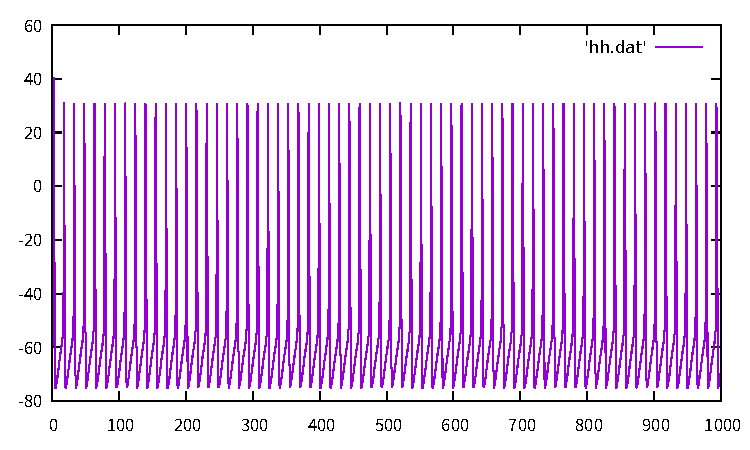
\includegraphics[width=0.45\textwidth]{./images/0301_hh_1000.pdf}
 \caption{スパイク発生の流れ} 
\end{figure}

\begin{thebibliography}{99}
\bibitem{lite1} 和田勝 ``筋肉による筋収縮の司令'' 生命科学C, 2001, https://www.tmd.ac.jp/artsci/biol/textlife/neuron.html.
% \bibitem{lite2} R. Hosaka, T. Kimura, and T. Matsuura, ``title,'' journal name, pp.10-20, 2021.
\end{thebibliography}
\end{document}
